\chapter{Implementation}
\label{ch:Implementation}

The implementation of PropertyIQ was based on the design decisions outlined in Section \ref{ch:Design} \nameref{ch:Design}, providing a comprehensive architecture and rationale for selecting XGBoost and SHAP, and integrating the models into the web application.

PropertyIQ is a compact system that comprises a data preparation pipeline, a valuation model, an explanation layer, a Python backend and a React frontend. The significance of this configuration lies in its dual focus: generate a valuation and ensure that this valuation is accessible and comprehensible to the user via the web application. 

The following subsections delineate the logical sequence of the system's construction. Commencing with the development environment and data preparation, progressing through feature engineering and model construction, and culminating in the integration of the back-end and front-end components.

\section{Project Structure and Development Environment}

The implementation of PropertyIQ was structured into three primary layers: a notebook-based machine-learning workspace, a Python backend, and a React frontend. This architecture was adopted at an early stage to facilitate project management and mitigate the risk of merging exploratory modelling and deployment-orientated tasks. 

Initially, the machine learning pipeline was developed within Jupyter Notebook, allowing inspection, cleaning, transformation, and use of the data set to train the regression model, which, consequentially, was used by the explanatory model to articulate the prediction. Once this component achieved sufficient stability, the trained artefacts (in the form of \texttt{.pkl} files \parencite{Oderinwale2025}) were transferred to the backend, allowing their use by the web application.

The development of the model involved iterative experimentation with data preprocessing steps, feature selection, and model configuration. By maintaining the training process within a notebook and the deployment logic in separate Python files, the model was refined without demanding the continual restructuring of large sections of the codebase upon changes.

The frontend was developed using React in combination with Vite, Tailwind CSS, React Router, and Recharts. The backend was implemented using FastAPI \parencite{FastAPI2025} and deployed via Uvicorn. Throughout both the backend and notebook phases, Pandas was employed to process, manage, and manipulate the data.


\section{Dataset and Data Preprocessing}

The initial phase of implementation focused on \textbf{transforming the data inside to be suitable for supervised machine learning}, as the dataset was sourced from scraped Zoopla listings and contained 1,000 rows and 43 columns in its raw form.

Although the data provided a valuable real-world basis for the project, they also introduced typcical challenges associated with data sliced on the web \parencite{Foerderer2023}. A significant number of fields were irrelevant, some were only partially populated, and several values that were inherently numerical were extracted as formatted strings.

The analysis started by importing the CSV dataset file into Pandas and performing an initial examination. This initial assessment promptly indicated that not all available fields would be advantageous for modelling purposes.

Certain columns, such as web URLs, image links, and map references, lacked direct relevance for price prediction \parencite{Kotsiantis2006}. Furthermore, some columns, including \texttt{virtual\_tours}, \texttt{deposits} and \texttt{letting\_arrangements}, were nearly empty of data; thus a more selective data filtering approach was adopted, focusing on fields that could be consistently cleaned and were likely to contribute meaningfully to the ML model valuation task.

A significant component of this phase involved the transformation of string-represented values into numerical counterparts. For example, the variable \texttt{price} was initially presented as a formatted string containing currency symbols and commas, while \texttt{service\_charge} was similarly formatted as an annual, monthly, or weekly amount, and \texttt{property\_size} included unit text rather than a simple number. 

These elements were processed using regular expression-based stripping before conversion into numerical values. In addition, fields such as the number of bedrooms, bathrooms, receptions, and leasehold-related attributes were converted to numerical form where feasible.

Furthermore, certain features, such as \texttt{property\_type}, were standardised to a lowercase value for subsequent encoding (e.g. ``new-homes'' are represented by \texttt{0} and ``for-sale'' by \texttt{1}). Although these procedures were not particularly complex from an algorithmic perspective, they were essential because the model could not be effectively trained on raw scraped text values.

Once the key variables were converted, records that were missing critical fields needed for training were removed, in particular, price and property size. This reduced the working dataset from 1,000 properties to \textbf{977 meaningful property records}. Although this meant losing a small part of the original data set, it improved the integrity of the training data and avoided building the core valuation model around incomplete records. 

In practice, this was one of the clearest examples of implementation being different from the initial ambition: the raw dataset appeared broad and information-rich at first glance, but only part of it was suitable for a stable ML model pipeline.


\section{Feature Engineering}

After the raw fields had been cleaned, the next stage was to \textbf{build a feature set that consisted of more meaningful data for the model than the raw dataset alone}. This was a key part of the implementation because the quality of the eventual valuation depended just as much on how the data were represented as on the model choice itself. 

At this point, it was necessary to move from simply cleaning values to constructing a representation of characteristics that could capture both the characteristics of the property and some of the wider context that affects the price, as described in the Appendix \ref{ch:Specifications} \nameref{ch:Specifications}.

Given the data already present, three new ``features'' were incorporated into the data.

\begin{enumerate}
    \item \texttt{price\_per\_sqft} is derived as 
    \begin{equation}
        \frac{\text{price}}{\text{size (sqft)}}
    \end{equation}
    capturing the density of value rather than absolute magnitude alone. This enables the model to make meaningful comparisons across properties of  varying sizes; for example, two properties priced at \pounds 300,000 may differ substantially in value if one spans 800 sqft and the other 1,200 sqft, a distinction that raw price and size alone would not convey \parencite{PermataHati2025}.

    \item \texttt{log\_price} is derived as 
    \begin{equation}
        \ln(1 + \text{price})
    \end{equation}
    and was introduced to address positive skewness in the price distribution, mitigating the disproportionate influence of high-value outliers on model training; by using Numpy function \text{log1p(price)}.
    In practical terms, a property listed at £5,000,000 would otherwise exert far greater weight than the majority of listings clustered below £500,000. Applying the logarithmic transformation compresses this range, promoting training stability. The predictions must then be inversely transformed by $e^{log\_price} - 1$ to recover interpretable price estimates \parencite{Veen2023} \parencite{Rico-Juan2021}.

    \item The address $a$ is mapped to a binary region indicator vector via a three stage pipeline: a regular expression extracts the alphabetic postcode prefix $p$ (e.g.\ \texttt{SW} from \texttt{SW1A 1AA}); a lookup $\phi$ maps $p$ to one of the $K = 23$ named regions $\mathcal{R} = \{r_1, \ldots, r_K\}$, falling back to the first character if the full prefix is not matched, or assigning a residual $r_{\text{other}}$ otherwise; a one-hot encoder $\psi$ produces the final feature vector

    \begin{equation}
        \Bigl(\mathbf{1}\bigl[\phi(\text{prefix}(a)) = r_k\bigr]\Bigr)_{k=1}^{K}
        \;\in\; \{0,1\}^{K}
    \end{equation}

    \noindent Mutual exclusivity is guaranteed by construction: $\sum_{k} \mathbf{x}_{\text{region}}(a)_k \leq 1$ for all $a$, providing the model with a structured locational signal reflecting geographic variation in property values in the UK \parencite{Kopczewska2022} \parencite{Rico-Juan2021}.
    
\end{enumerate}

Collectively, these feature engineering decisions address three fundamental challenges in training a 
machine learning model on property data. 

First, \texttt{price\_per\_sqft} ensures that the model captures relative value rather than absolute figures, reducing the risk of size-driven bias in its predictions \parencite{PermataHati2025}. Second, the logarithmic transformation of price stabilises the target distribution, preventing a small  number of high-value outliers from disproportionately skewing the learnt parameters \parencite{Veen2023}; a particularly important consideration given the wide price range typical of UK housing markets. Third, the one-hot encoded postcode features introduces structured geographic context, allowing the model to account for locational variation without imposing an arbitrary ordinal relationship between regions \parencite{Kopczewska2022}, given that different areas have different property values, the models ``clusters'' the different properties by area and account for the property location when making a valuation, as shown in Figure \ref{fig:distribution}.

\begin{figure}[h]
    \centering
    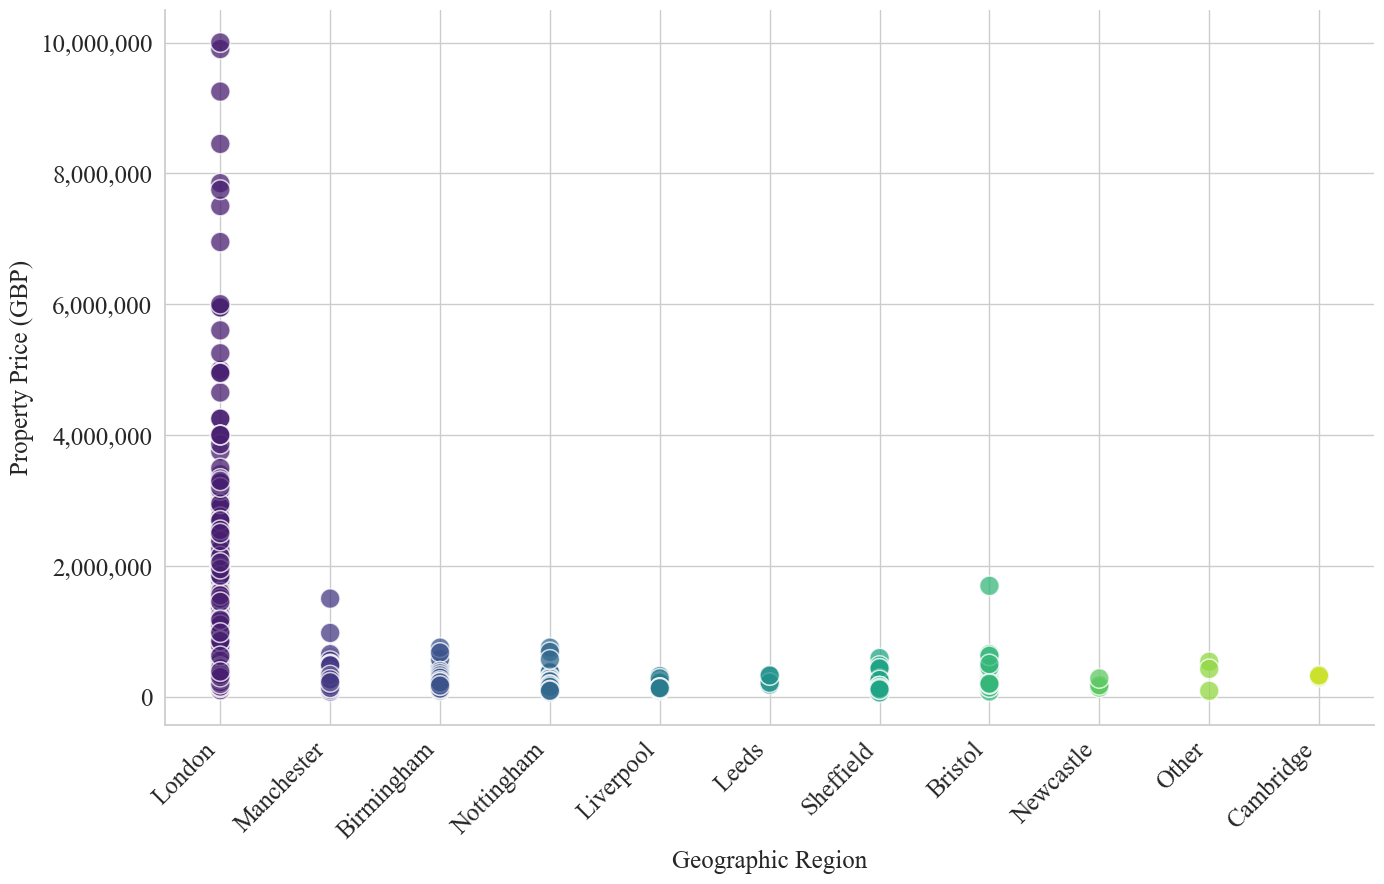
\includegraphics[width=\textwidth]{impl/images/distribution.png}
    \caption{Properties Prices distributed by Region.}
    \label{fig:distribution}
\end{figure}

Together, these transformations \textbf{reduce noise, improve distributional assumptions, and provide the model with richer, more discriminative inputs}; all of which contribute to more accurate and generalisable predictions across diverse property types and locations.


\section{Model Training and Evaluation}

With the cleaned and engineered feature set in place, the valuation model for properties prices using XGBoost was implemented.

The model was trained to predict the logarithmic value of the price of the property, using the processed features as input. Data were split using standard 80\% training and 20\% testing split returned from \verb|sklearn.model_selection.train_test_split| \parencite{ScikitLearn2025}.

With \verb|random_state=42| \parencite{Ahmed2022} used to keep the split reproducible between repeated runs. This was helpful during development because it meant that changes in performance or behaviour could be traced back to changes in the pipeline itself rather than differences in the train-test split. The final model was implemented as an \texttt{XGBRegressor} \parencite{DistributedDeepMachineLearningCommunity2026} with a \texttt{random\_state=42}, making the model reproducible.

\begin{minted}[
    bgcolor=gray!8,
    linenos=true,
    fontsize=\small,
    frame=single,
    rulecolor=gray!40
]{python}
from xgboost import XGBRegressor

model = XGBRegressor(
    n_estimators=500,
    learning_rate=0.05,
    max_depth=8,
    subsample=0.8,
    colsample_bytree=0.8,
    random_state=42,
    eval_metric='rmse'
)
\end{minted}

These parameters were not determined through exhaustive searches of all possible combinations. Although a more comprehensive tuning process could have been conducted, it would have significantly increased the time required without necessarily altering the broader contribution of the project, which relies as much on explainability and integration as on raw predictive optimisation. 

Moreover, such extensive tuning was unnecessary because the default parameter configuration already yielded a high-level \textbf{estimating model with an accuracy of 0.9557}.

Upon completion of the final model training, both the regression trained model and the feature column list were preserved as \verb|pickle| files. The preservation of both files is essential for the explanatory SHAP model and for the web application prediction architecture.

This approach facilitated a clear delimitation between the notebook-based training phase and the web application layer. Consequently, the backend loads the saved artefacts, eliminating the need to re-execute the training code or reconstruct the training environment during runtime.

Although the notebook also includes held-out testing and metric calculation, the results are addressed in the relevant Chapter \ref{ch:Evaluation} \nameref{ch:Evaluation}.

\section{SHAP Explanation Layer}
\label{se:SHAPExplanationLayer}

The explanation pipeline was implemented across two components: the module encapsulating the core 
inference and attribution logic, and the dedicated route exposing this functionality to the frontend. 
The explainer loads the persistent XGBoost model along with the stored feature column list, reconstructs the input feature vector from a dictionary of property attributes, and applies \verb|shap.TreeExplainer|\parencite{shap2026} to generate local feature-attribution values for each prediction.

A critical requirement during this phase was to ensure that the inputs supplied at deployment were subjected to identical preprocessing to that applied during training. This included reconstructing one-hot encoded columns for postcode area and property type, inserting any absent columns as zeros, and reordering the feature vector to match the training schema; which is defined inside the \verb|predict_and_explain(input_features: dict)| function. Failure to enforce this consistency would have compromised the reliability of the SHAP attributions and would risk producing erroneous output. 

Consequently, a substantial portion of the explanation logic is dedicated to input validation and structural reconstruction, rather than the attribution computation itself.

A further consideration concerns the presentation of SHAP outputs to end users. Raw feature-attribution values, whilst informative for technical inspection, are not readily interpretable by a general audience, and thus, by the end users of this project. To address this, the system was designed to return both the underlying SHAP contribution values and a concise natural-language summary of the prediction rationale. This translation layer between the technical attribution output and the user-facing interface was a deliberate design decision, intended to \textbf{improve the accessibility and interpretability of the system without sacrificing the underlying analytical depth}.


\section{Backend Implementation}

Once the valuation and explanation components were functioning reliably, a FastAPI backend was implemented through Uvicorn and it acted as the primary connection point between the machine learning pipeline and the frontend web application. Its role was to serve listing data from the CSV dataset, load the persisted model artefacts, accept property inputs from the web application, and return predictions and explanations.

The main backend file is \verb|app.py|, which defines the FastAPI application, request schema, utility functions, and API routes. In addition, a \verb|PropertyInput| class was used to specify the fields expected for prediction and explanation requests, based on the features that were used during the training of the XGBoost regression model. In practice, using a defined request model improved consistency and made testing easier because the API always expects a stable structure.

The backend architecture incorporates distinct routes, namely \verb|/predict| and \verb|/explain|. The \verb|/predict| route exclusively returns the predicted value for a property given the features that make up it, whereas the \verb|/explain| route provides a comprehensive output, including the predicted value, the base price, the SHAP breakdown and concise human-readable explanatory text.

Additional routes were implemented to facilitate direct access to the properties records in the dataset, specifically \verb|/api/properties|, \verb|/api/property/{uprn}| requiring the Unique Property Reference Number (UPRN) and \verb|/api/risk-data-csv|. These routes were instrumental in supporting the frontend browsing, detail view, and risk analysis functionalities, allowing the system to function beyond a mere prediction endpoint.

Together, these components established a structured and extensible backend architecture capable of serving both predictive and explanatory outputs alongside raw listing data, forming the foundational communication layer between the machine learning pipeline and the deployed PropertyIQ web application.


\section{Frontend Implementation}

The final implementation phase concerned the development of the frontend, which translated the backend functionality into an accessible web application. The interface was constructed using React and Vite, organised as a single-page routed application with dedicated views for the dashboard, property listings, analysis, property details, and a system explanation page. This structure reflects the overarching objective of this project as a decision-support tool rather than a purely predictive demonstration.

Navigation between views was managed through the React Router, whilst Axios\parencite{Axios2025} facilitated communication with the backend API. Tailwind CSS was used for rapid interface development, and Recharts was used where visual representations offered greater clarity than textual or tabular alternatives. The dedicated explanation page was of particular significance, as it surfaces the underlying system architecture to the user rather than concealing the decision-support process behind the interface, a choice that directly reinforces the transparency objectives of this project.

Certain elements of the initial specification were refined during development, most notably the range of features used for modelling and the complexity of the generated explanatory text. These adjustments were pragmatic in nature and did not compromise the fundamental scope of the project. The resulting system successfully achieved its central objective by integrating property valuation with explainability in a functional, demonstrable artefact, fulfilling the requirements of providing predictive functionality through a backend API and presenting results through a browser-based interface.
